\chapter{Dijkstra's shortest paths algorithm}
\lecture{1}{20/1}

We can represent a graph using an \textbf{adjacency matrix};
the entry in row $i$ and column $j$ is
\begin{enumerate}
    \item $w$ if there is an edge of weight $w$ from $i$ to $j$; and
    \item $0$ if there is no edge.
\end{enumerate}

\begin{figure}
    \centering
    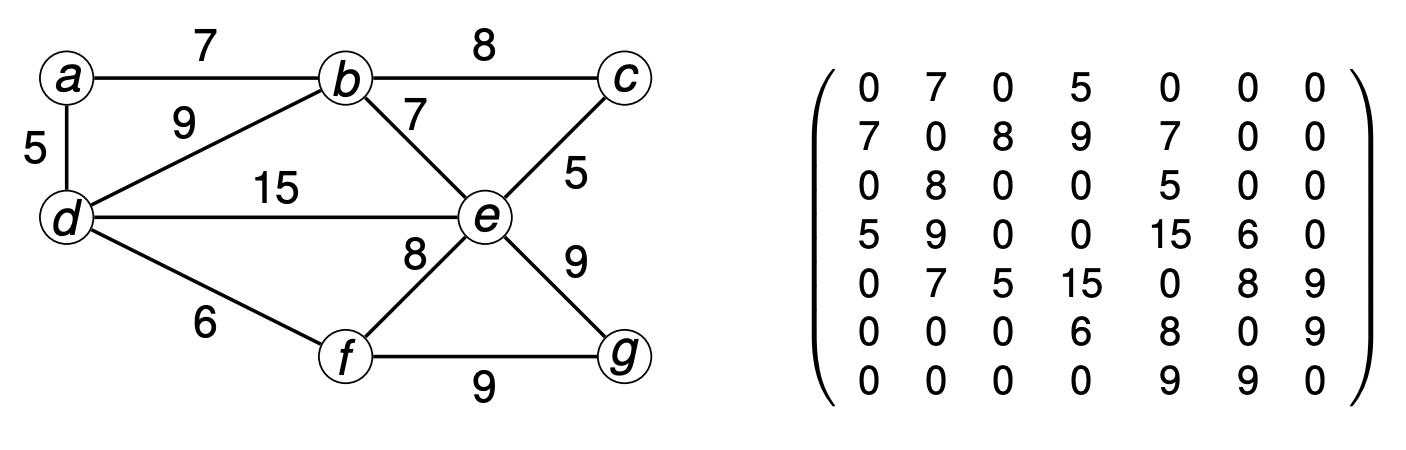
\includegraphics[width=0.8\linewidth]{images/adj-matrix.png}
    \caption{A graph with the adjacency matrix representation.}
    \label{fig:adj-matrix}
\end{figure}

The \textbf{weight} of a path from a vertex $u$ to a vertex $v$ is the
sum of the weights of the edges in the path.
Note that a weight may be negative. 
We will be looking at \emph{directed} graphs.

The \textbf{shortest path} between vertices $u$ and $v$ is denoted 
$\delta(u, v)$.
If no path exists then $\delta(u, v) = \infty$. 

We call a directed cycle
\begin{enumerate}
    \item \textbf{positive}, if its edge weights sum up to a positive number; and 
    \item \textbf{negative}, if its edge weights sum up to a positive number.
\end{enumerate}

A positive cycle will never be contained within the shortest path between two 
vertices.
However, if there is a negative cycle between vertices $u$ and $v$ then
$\delta(u, v) = -\infty$.

Our aim is to find an algorithm that solves the single-source shortest paths
problem; that is, an algorithm that finds the shortest path from a specific 
source vertex $s$ to all other vertices in the graph.
This is a generalisation of breadth-first search, where every edge weight is set
to $1$. The output of our algorithm will be two arrays $d$ and $\pi$ where for
each vertex $v$:
\begin{enumerate}
    \item $d(v) = \delta(s, v)$; and
    \item $\pi(v)$ is the \emph{predecessor} of $v$.
\end{enumerate}

First, we will assume the problem such that all weights are non-negative.
We do not directly computer $d(v) = \delta(s, v)$ in contrast to BFS,
instead at each step $d(v)$ is an estimate for $\delta(s, v)$.
Initially $d(v) = \infty$ and we always have $d(v) \geq \delta(s, v)$.
$d(v)$ is decreases as shorter paths are found, at the end of the algorithm we
have $d(v) = \delta(s, v)$.

The process of \emph{relaxing} an edge $(u, v)$: 
first we check whether the shortest path going from $s$ to $v$ can be 
improved by going through $u$, 
if so we update our $\delta$ and $\pi$.

Then Dijkstra's algorithm can be found

\begin{algorithm}
    Bottom-up dynamic programming for paranthesis positioning.
    \begin{algorithmic}[1]
        \Procedure{InitialiseSingleSource}{$G$, $s$}
            \For{$v \in G$}
                \State $d(v) \gets \infty$
                \State $\pi(v) \gets \text{nil}$
            \EndFor
            \State $d[s] \gets 0$
        \EndProcedure
        \Procedure{Relax}{$u$, $v$, $w$}
            \If{$d(v) > d(u) + w(u, v)$}
                \State $d(v) = d(u) + w(u, v)0$
                \State $\pi(v) = u$
            \EndIf
        \EndProcedure
        \Procedure{Dijkstra}{$G, w, s$}
            \State $\text{\textsc{InitialiseSingleSource}}(G, s)$
            \State $S \gets \emptyset$
            \State $Q \gets V(G)$
            \While{$Q \neq \emptyset$}
                \State $u \gets \operatorname{PopMinimum}(Q)$
                \State $S \gets S \cup \{u\}$
                \For{$v \in \operatorname{Adj}(u) \setminus S$}
                    \State $\operatorname{\textsc{Relax}}{(u, v, w}$
                \EndFor
            \EndWhile
        \EndProcedure
    \end{algorithmic}
\end{algorithm}

Initialisation takes $O(V)$ times as there is two operators per vertex,
finding the minimum vertex takes $O(V)$ and is done $V$ times and so
total $O(V^2)$, and relaxation takes in total $O(E)$ times as every
edge is relaxed once. Therefore, the total running time is
\[ O(V + V^2 + E) = O(V^2). \]
However, there is optimisations related to how we find the minimum
value (heaps) that make Dijkstra's more efficient; that is, it runs in
\[ O(V\log V + E). \]

\begin{proposition}[Properties of shortest paths and relaxation]
    \hfill
    \begin{enumerate}
        \item For all edges $(u, v)$, we have
            \[ \delta(s, v) \leq \delta(s, u) + w(u, v). \]

        \item Any subpath of a shortest path is also a shortest path.

        \item For every vertex $v$, we always have $d(v) \geq \delta(s, v)$.

        \item If $\delta(s, v) = \infty$, then we have $d(v) = \infty$ 
            at every iteration.

        \item If there is a shortest path from $s$ to $v$ including the
            edge $(u,v)$ and if $d(u) = \delta(s, u)$,
            then we obtain $d(v) = \delta(s, v)$ when $(u, v)$ is relaxed.
    \end{enumerate}
\end{proposition}

To prove the correctness of Dijstra's, we need to prove that the loop ionvariant always remains true.

At the start of each iteratino of the while look, $d(v) = \delta(s, v)$ for every $v \in S$.
\begin{enumerate}
    \item At the start of the algorithm $S$ is empty, so the loop invariant is trivially true.
    \item Maintenance: we need to show that $d(u) = \delta(s, u)$, when $u$ is added to $S$.
    \item Termination: at the end, $S$ contains every vertex, which implies that 
        $d(v) = \delta(s, v)$ for all vertices $v$ in the graph.
\end{enumerate}
